\chapter{COVID-19 Analysis}
\setcounter{secnumdepth}{5}
\label{ch:AI}
\setlength\lineskip{0pt}
\vspace*{15pt}

\definecolor{codegreen}{rgb}{0,0.6,0}
\definecolor{codegray}{rgb}{0.5,0.5,0.5}
\definecolor{codepurple}{rgb}{0.58,0,0.82}
\definecolor{backcolour}{rgb}{0.95,0.95,0.92}
\definecolor{deepred}{rgb}{0.6,0,0}
 
\lstdefinestyle{mystyle}{
    backgroundcolor=\color{backcolour},   
    commentstyle=\color{codegreen},
    keywordstyle=\color{blue},
    numberstyle=\tiny\color{codegray},
    stringstyle=\color{codepurple},
    basicstyle=\footnotesize,
    breakatwhitespace=false,         
    breaklines=true,                 
    captionpos=b,                    
    keepspaces=true,                 
    numbers=left,                    
    numbersep=5pt,                  
    showspaces=false,                
    showstringspaces=false,
    showtabs=false,                  
    tabsize=2
}
 
\lstset{style=mystyle}

During Chapter \ref{ch:progress}, we had the opportunity to understand how to possibly model a disease spreading in a community. In this chapter, we are instead going to expand this topic in order to take into account how the spreading of the disease can be forecasted (using real world data) and how clinical trials and comorbodities can be taken into account in the case of COVID-19.

\section{SIR Time Series Estimation}
Building on from the SIR model constructed in Section \ref{sir_sec}, we can then make use of it in order to approximate real world data and predict future trends \cite{atom}.

This process can be summarised in the following two steps:

\begin{enumerate}
    \item Estimating $\beta$ and $\gamma$, given the data about the number of cases and recovered in a country. In order to optimise iteratively these two parameters, has been made use of a modified form of the Root Mean Squared Error (RMSE) equation to take into account of both the number of cases series and the number of recovered individual (Equation \ref{loss_it}). In Equation \ref{loss_it}, has additionally added an hyper-parameter ($\alpha$) to decide if to give more weight either to optimising the cases or recovered curve fit. This exercise has therefore been designed to be an optimization minimization problem, in which the parameters estimation is improved iteratively by minimising the overall loss. This optimization process is then carried out making use of the Limited-memory BFGS (L-BFGS) algorithm. The L-BFGS algorithm, is an approximation\footnote{Limited-memory BFGS, approximating the traditional BFGS algorithm manages to in fact to keep a linear memory consumption.} of the traditional BFGS (Broyden–Fletcher–Goldfarb–Shanno algorithm) algorithm which works by estimating the Inverse of the Hessian Matrix in order to move through the search space. The calculated $\beta$ and $\gamma$, are then going to be used as our parameters for the SIR model.
    
    \useshortskip
    \begin{align}
    \ Loss = \alpha \times \sqrt{\dfrac{1}{n} \sum_{t=1}^{n} (I_{t} - ID_{t})^{2}} + (1 - \alpha) \times \sqrt{\dfrac{1}{n} \sum_{t=1}^{n} (R_{t} - RD_{t})^{2}}
    \label{loss_it}
    \end{align}
    \vspace{-0.4cm}
    \begin{conditions}
     $I_{t}, R_{t}$  &  SIR Infected and Recovered timestep \\
     $ID_{t}, RD_{t}$  &  Infected and Recovered from data timestep \\
     $n$  &  Number of timesteps\\
    \end{conditions}
    \vspace{-0.2cm}
    \useshortskip
    \item Solve the SIR model equations by numerically integrating them and providing some initial condition values for the number of susceptible, infected and recovered in the population. The values of the initial conditions, can then be calculated by taking into account the population size of the country we are examining and the number of cases registered so far. The integration method used instead to solve the system of differential equations ($4^{th}$ order for 3 dimensions), was the Explicit Runge-Kutta method \cite{kutta}.
\end{enumerate}


In Figure \ref{sir_forecast}, are available the prediction results of Italy and Germany as of the $9^{th}$ of July 2020 in order to predict the following 30 days trends. As can been seen from the results, both countries have been fairly well approximated and the number of infected predicted in the simulation have been slightly overestimated. This mismatch although, can still look quite realistic in real life because of the limited amount of tests available and presence of asymptomatic patients.

% \vspace{-0.1cm}
\begin{figure}[ht!]%
    \centering
    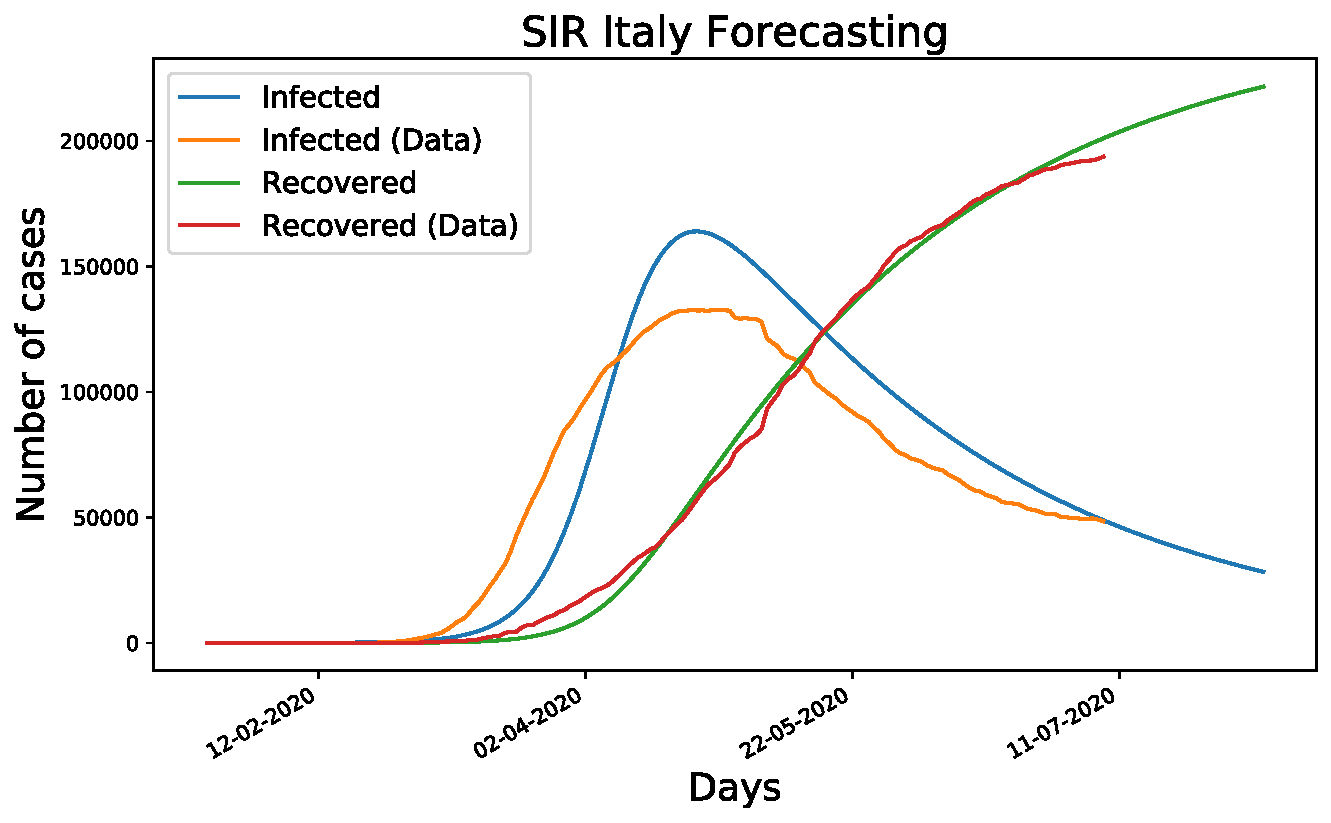
\includegraphics[width=0.49\linewidth]{latex/images/Italy_preds.pdf}
    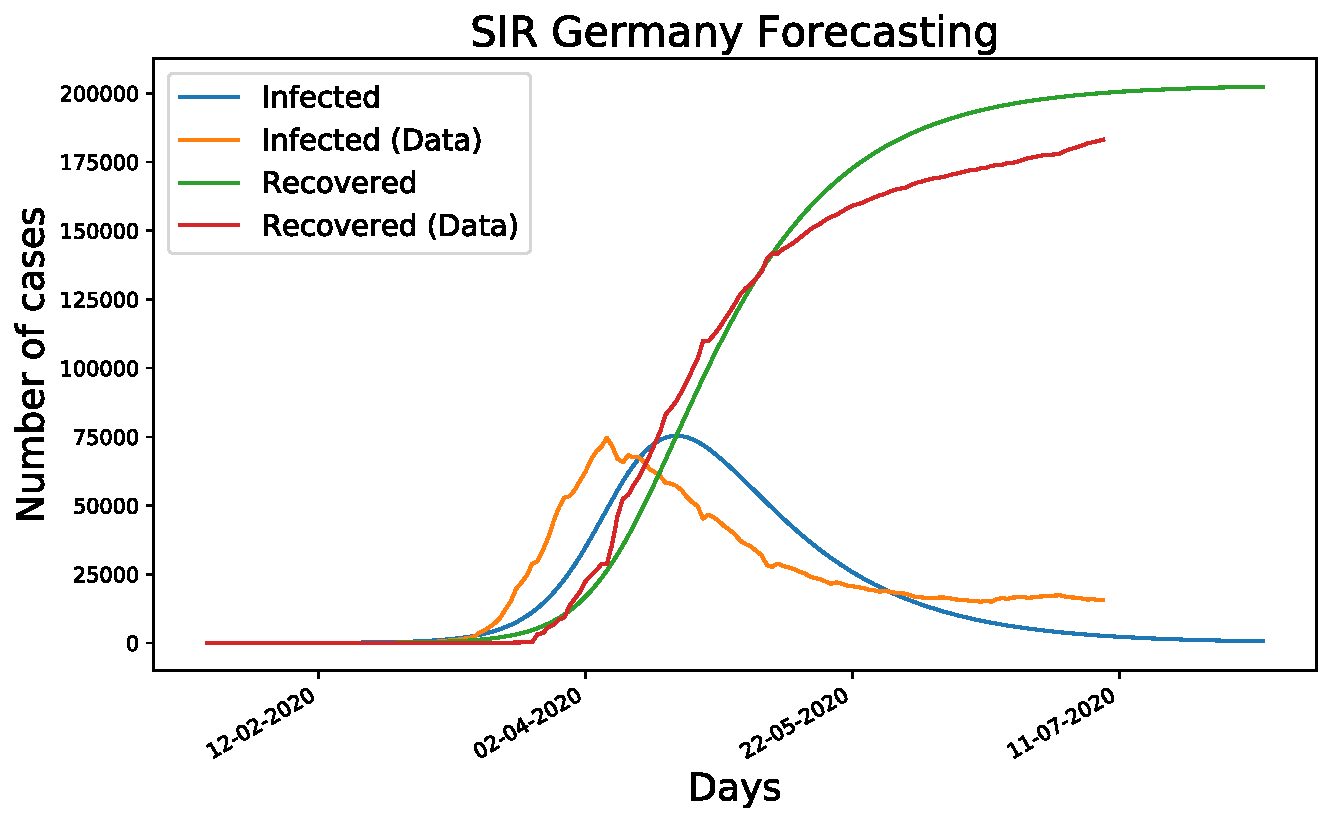
\includegraphics[width=0.49\linewidth]{latex/images/Germany_preds.pdf}
    % 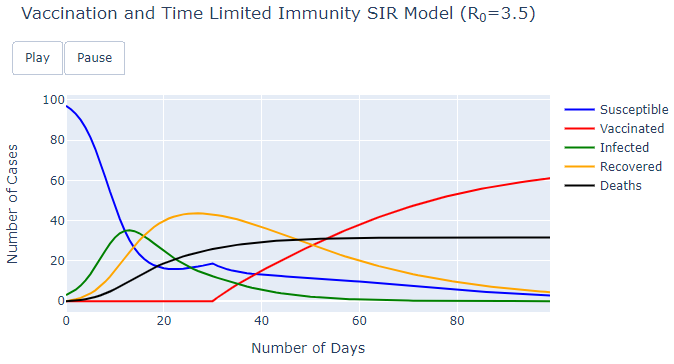
\includegraphics[width=13cm]{latex/images/vacc.PNG}%
    \vspace{-0.2cm}
    \caption{Italy and Germany SIR Forecasting}
    \label{sir_forecast}
\end{figure}
% \vspace{-0.1cm}

\subsection{ML Forecasting}

Another possible approach which can be taken in order to forecast time series, is to use standard Machine Learning and Deep Learning techniques. In this case, the number of infected cases in Germany over time is going to be taken as example \footnote{Using data up to the $9^{th}$ of July 2020.} in order to forecast the number of cases in 30 days time. 

In order to accomplish this task, has been made use of the Python Darts library \cite{darts} and the following models have been taken into consideration:
\begin{enumerate}
    \item \textbf{Auto ARIMA (Auto Regressive Integrated Moving Average)}: is a time series method which can be used in order to make predictions as a linear weighted sum of past input data. In the Auto version of the ARIMA, the model parameters are automatically inferred through differencing tests and optimised by recording Information Criterion (e.g. Akaike Information Criterion (AIC)) metrics.
    \item \textbf{Exponential Smoothing}: this technique follows the same approach of standard ARIMA models, but the model assigns exponentially decreasing weights for past observations.
    \item \textbf{LSTM (Long-Short-Term-Memory)}: The LSTM is a type of Recurrent Neural Network (RNN) ideated in order to add a memory mechanism suitable to analyse time series (the information is kept in a loop and data is fed in sequentially).
    \item \textbf{T-CNN (Temporal Convolutional Neural Network)}: The T-CNN is a type of Convoluational Neural Network used for time series forecasting. This type of model is composed by a one dimensional convoluational network combined with causal convolutions. In causal convolutions, outputs at a specific timestep are convolved just with elements of the same timestep and of previous layers (in order to add time dependencies).
\end{enumerate}

The results obtained from this analysis are available in Figure \ref{ml_forecast}. In this case, all the models have been used in order to predict a portion of the current series (so that to estimate a fit loss) and predict the next 30 days in the future of number of cases in Germany.

% \vspace{-0.1cm}
\begin{figure}[ht!]%
    \centering
    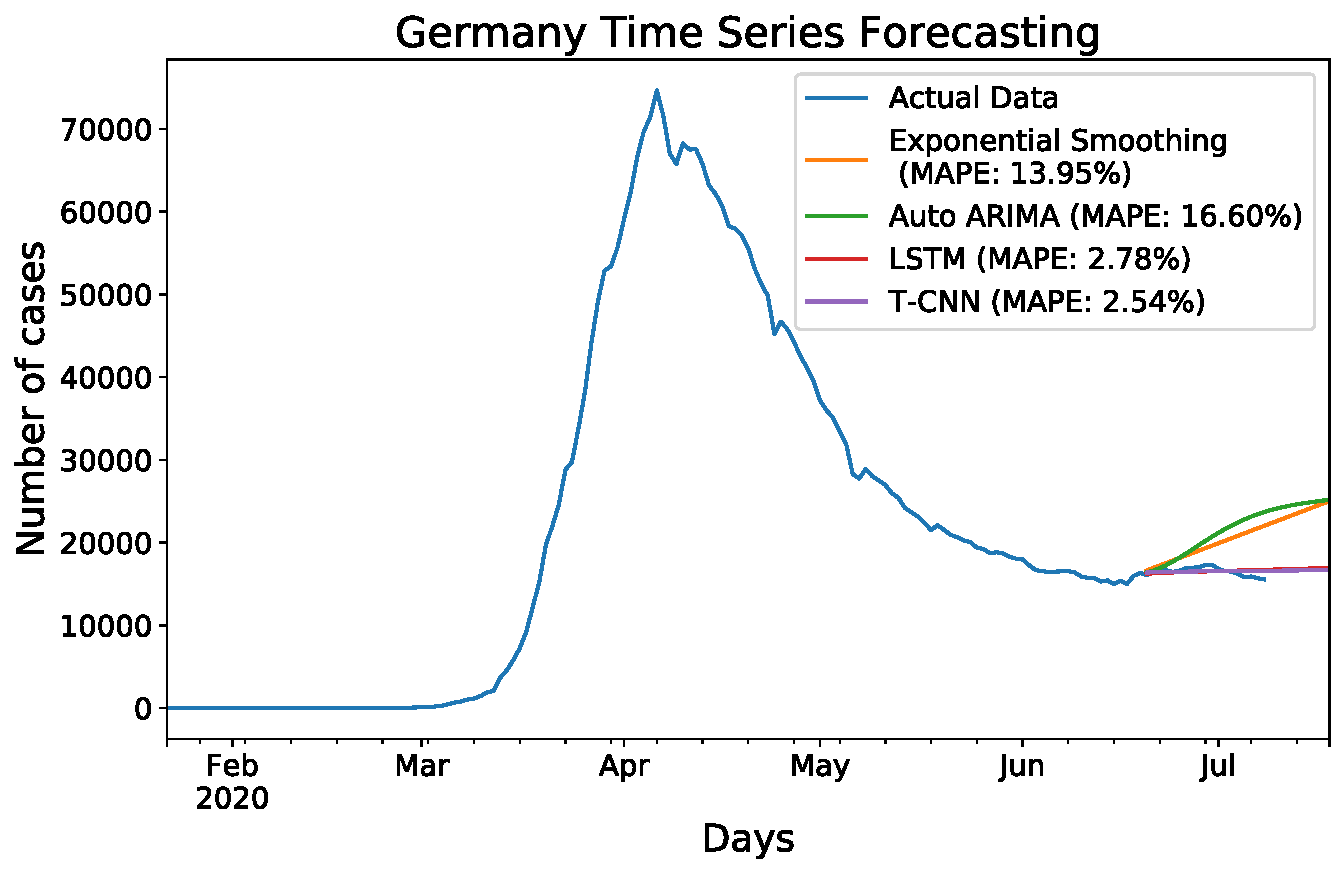
\includegraphics[width=0.55\linewidth]{latex/images/Germany_darts.pdf}
    % 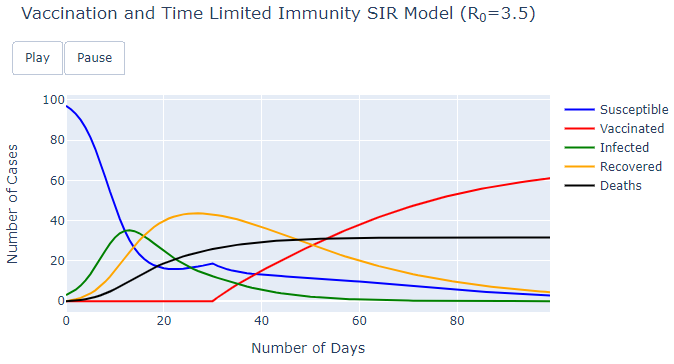
\includegraphics[width=13cm]{latex/images/vacc.PNG}%
    \vspace{-0.2cm}
    \caption{Germany ML Forecasting}
    \label{ml_forecast}
\end{figure}
% \vspace{-0.1cm}

In this case, has been decided to use MAPE (Mean Absolute Percentage Error) as our loss function. 
MAPE is in fact one of the most commonly used loss function for regression tasks, it's main advantages are interpratibility (we work using percentage terms) and scale-independency (Equation \ref{mape}). One of the main disadvantages of MAPE is that it can be undefined for actual values close to zero.

\useshortskip
\begin{align}
\ MAPE = \dfrac{1}{n} \sum_{t=1}^{n} \abs{\frac{A_{t}-F_{t}}{A_{t}}} \times 100
\label{mape}
\end{align}
\vspace{-0.4cm}
\begin{conditions}
 $A_{t}, F_{t}$  &  Actual and forecasted time-step \\
 $n$  &  Number of datapoints\\
\end{conditions}
\vspace{-0.2cm}
\useshortskip

Overall, the LSTM and T-CNN managed to best fit the original data, while both Exponential Smoothing and Auto ARIMA predicts and increase in the number of cases over the next month.

One of the major trade-offs in nowadays Machine Learning is model performance against complexity. In fact, complex Deep Learning architectures are usually able to perform better in a wide variety of tasks compared to traditional linear classifiers and regression techniques. This trade-off has been analysed in-depth in the 2016 publication "Why should I trust you?" by Ribiero et. al. \cite{exp_ai} and led a new trend in AI to focus on interpretability. Using for example, an SIR model in order to make predictions, can in fact allow us to now only to make estimates (like just done using ML based techniques), but also to infer underlying epidemology parameters such as $\beta$ and $\gamma$ which can in turn give us more information about how the disease is spreading.

% \section{Vector Autoregression}
\vspace{-0.2cm}
\section{Clinical trials}

Making use of the data for the United States ClinicalTrials.gov website, has been possible to gain insights about current clinical trials as of July 2020 against COVID-19 \cite{trials_data}. As can be seen from Figure \ref{trials}, Hydroxychloroquine had been so far the most common treatment tried.
\vspace{-0.2cm}
\begin{figure}[ht!]%
    \centering
    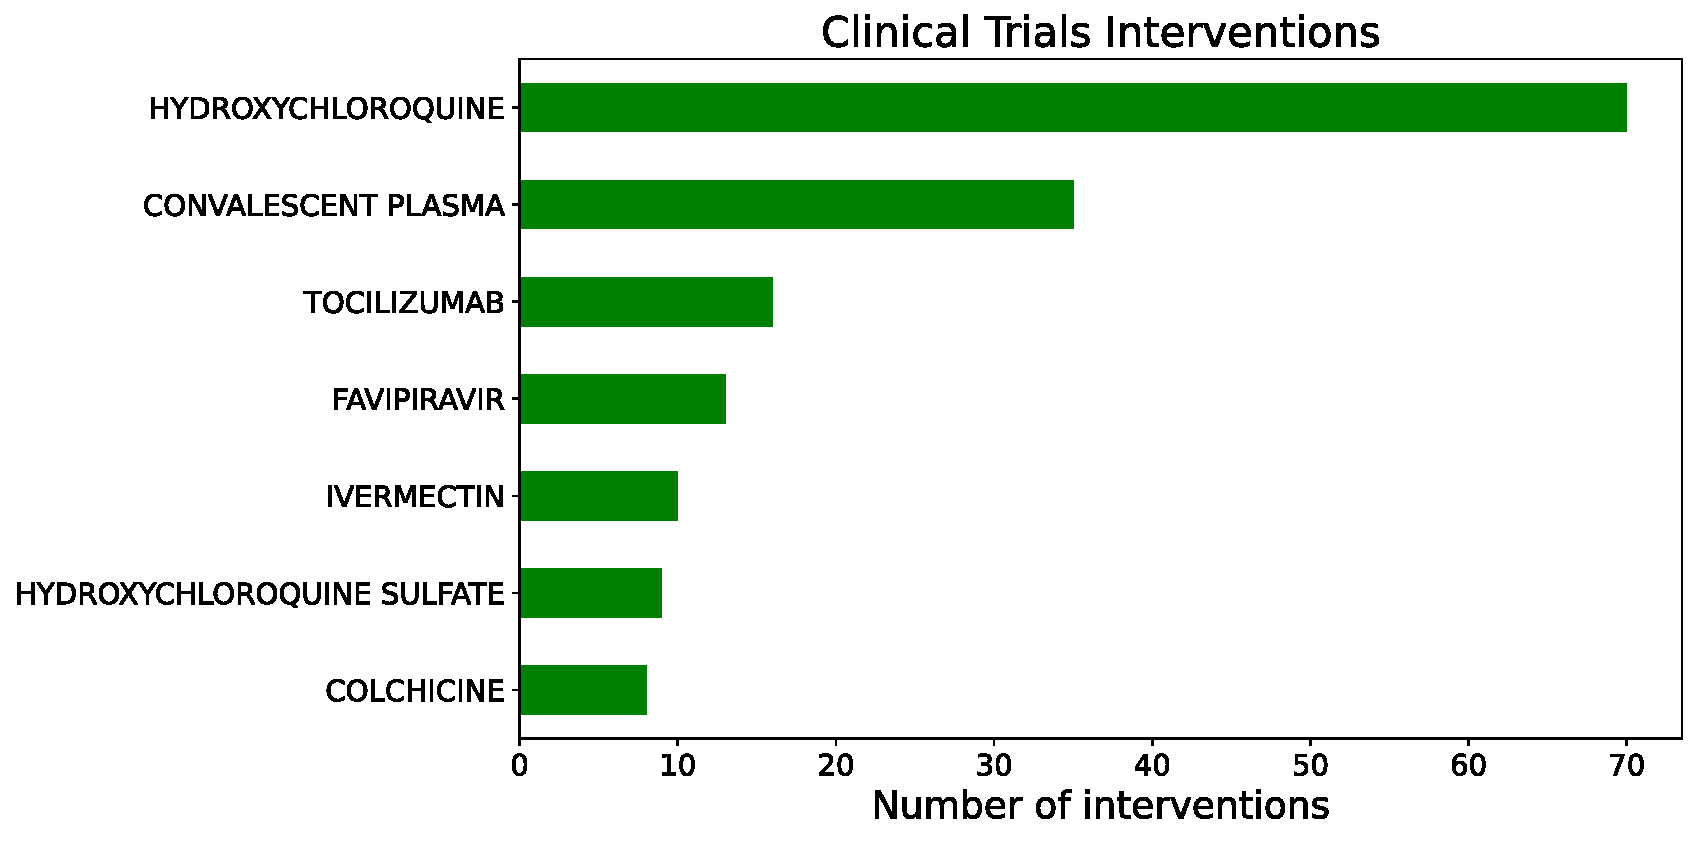
\includegraphics[width=0.65\linewidth]{latex/images/trials.pdf}
    % 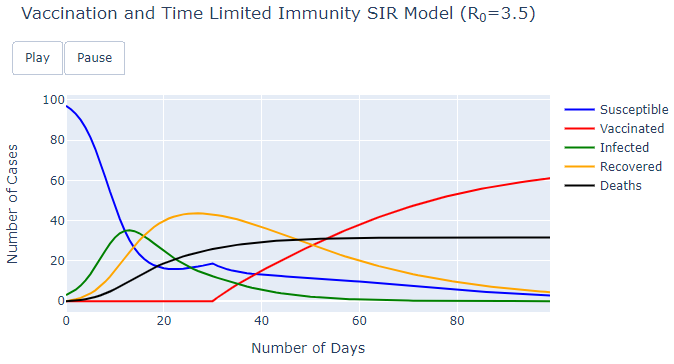
\includegraphics[width=13cm]{latex/images/vacc.PNG}%
    \vspace{-0.2cm}
    \caption{COVID-19 Clinical Trials}
    \label{trials}
\end{figure}
\vspace{-0.2cm}

As outlined in Section \ref{testing}, clinical trials are one of the main example of A/B testing application. Gathering results from an A/B test, we can then be able to infer causal relationships about what can be the potential effects of a treatment \cite{power}.

In this setting, the Causal question we are asking ourselves is: Does a certain treatment decrease COVID-19 mortality rate? This question, can then be formulated in statistical terms as a \textbf{null and alternative hypothesis}. In the null hypothesis, applying the treatment would not lead to any major change in the mortality rate and therefore both the treatment and control groups will be quite similar. Instead, in the alternative hypothesis, the treatment would cause a statistically significant change between the two groups. In our case, patients affected by COVID-19 would be considered as our population and our intervention (providing experimental medical treatment), would then be compared to no intervention. Variation in mortality rate could then be used our our metrics to asses the results. Patients should then be randomly assigned to either groups so that to avoid introduction of any form of bias (e.g. patients age, comorbidities, geographical location). If bias is unconsciously introduced, then this could lead to some form of \textbf{confounding bias}, which would then make really difficult to disconnect what are effects due to the intervention and which ones are instead caused a flow in the randomization process. 

Following on with our example, the number of times an intervention leads to a substantial difference compared to the control group, can then be summarised over a number of trials as a Binomial Distribution. In this distribution, the X axis will represent the count of possible outcomes, while the Y axis will represent the probability associated with an outcome. Although, according to the Central Limit Theorem, as we would increase our sample size, we would then end up with a Gaussian Distribution for each group in the experiment. In Figure \ref{test_dist}, is shown a possible outcome for our example. As can be see from the diagram, four different areas are present: True Positive (TP), True Negative (TN), False Positive (FP), False Negative (FN).
\vspace{-0.2cm}
\begin{figure}[ht!]%
    \centering
    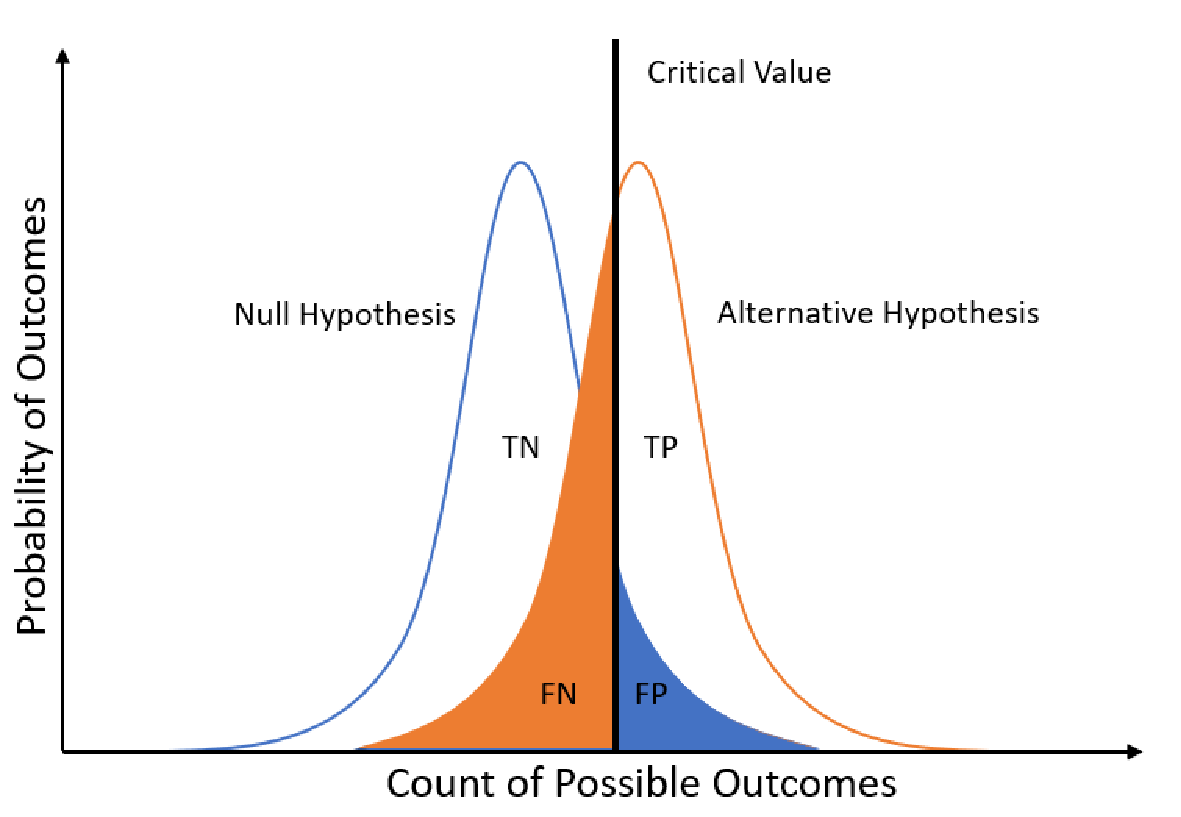
\includegraphics[width=0.6\linewidth]{latex/images/abtest.pdf}
    % 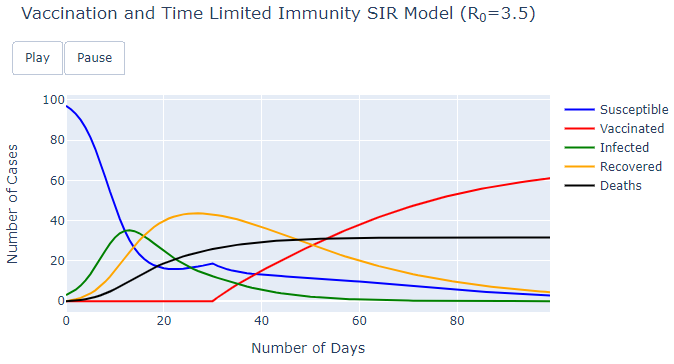
\includegraphics[width=13cm]{latex/images/vacc.PNG}%
    \vspace{-0.2cm}
    \caption{A/B Test Distributions}
    \label{test_dist}
\end{figure}
\vspace{-0.6cm}

In the TP case, we can affirm our treatment is beneficial since it managed to pass our test for the hypothesis (e.g. decreasing the mortality rate). In the case of the TN area, we can instead affirm that our treatment is not beneficial. While in the FP area, we might be deceived to believe our intervention was beneficial while it wasn't (the opposite holds true instead in the FN area). In these last two cases, it is then vital to look for any possible form of bias interference.

\section{Coronavirus comorbidities}

Two of the greatest factors, which seems to have the greatest impact over the mortality of Coronavirus for different patients, seems to be age and possible pre-existing conditions. In different models implemented in Chapter \ref{ch:progress}, has been taken into account of the age factor by varying the mortality likelihood depending on age. In this section\footnote{Making us of the data provided by the National Center for Health Statistics \cite{deaths_data}.}, we are instead going to give a look at which pre-existing conditions seems to have the greatest impact on COVID-19 mortality (Figure \ref{d_cond}). 

\begin{figure}[ht!]%
    \centering
    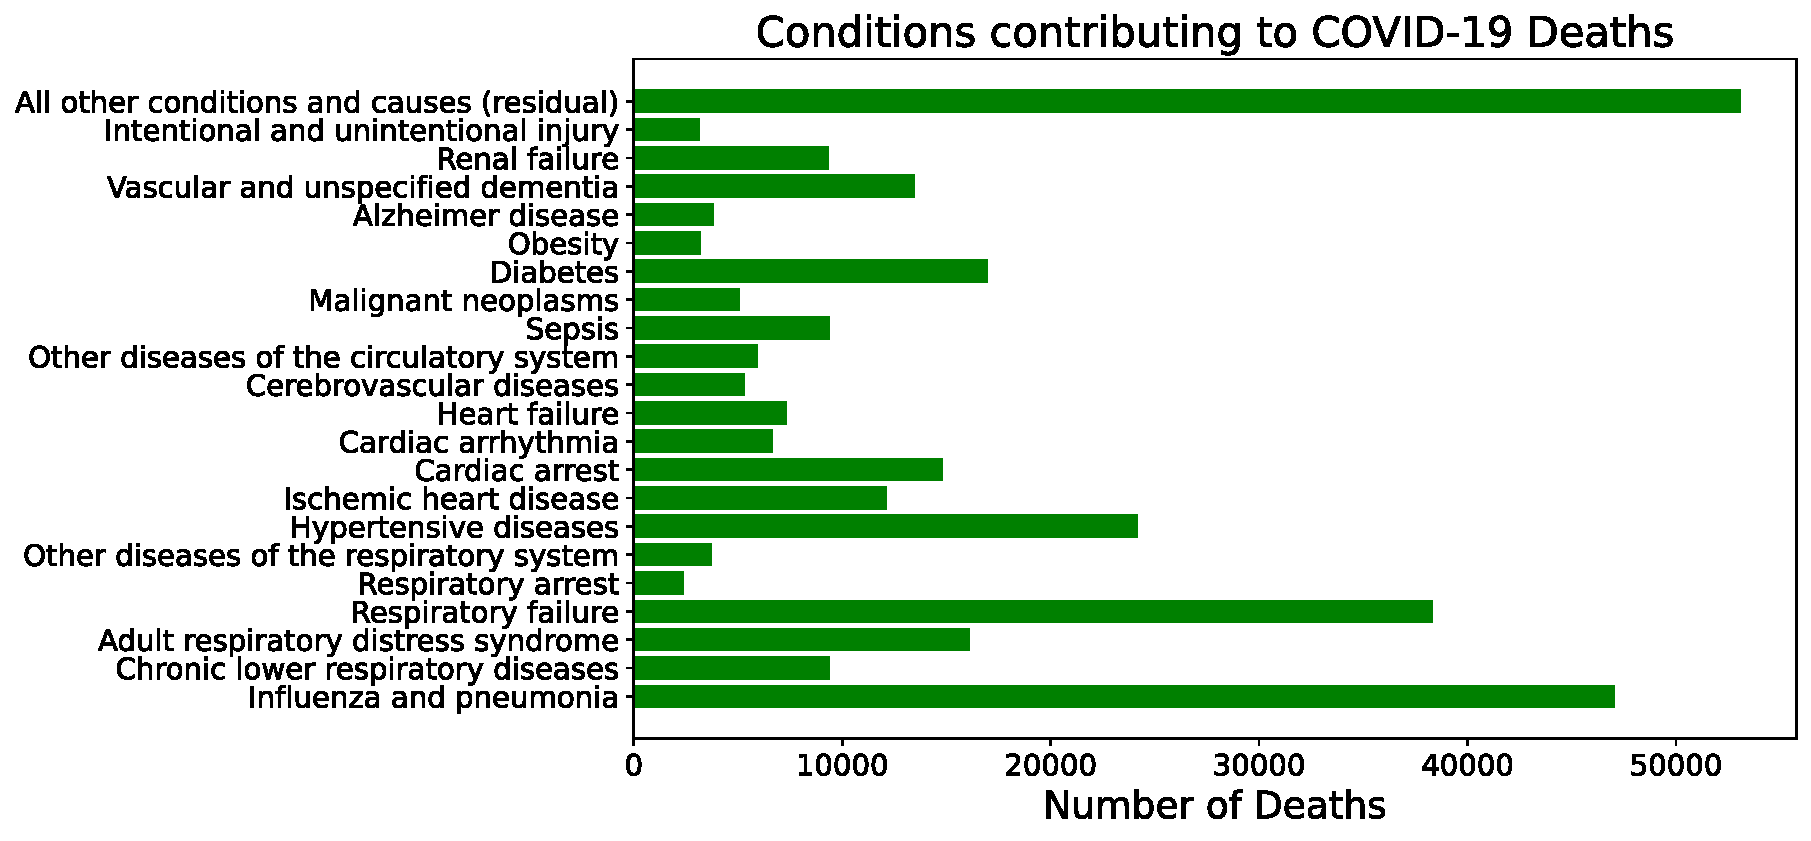
\includegraphics[width=0.85\linewidth]{latex/images/deaths_conditions.pdf}
    % 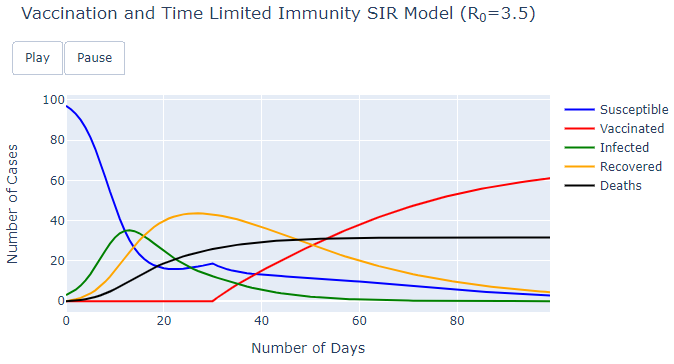
\includegraphics[width=13cm]{latex/images/vacc.PNG}%
    \vspace{-0.2cm}
    \caption{Conditions contributing to COVID-19 Deaths}
    \label{d_cond}
\end{figure}

As can be seen from \ref{d_cond}, Influenza and pneumonia seems to be one of the main causes of deaths related to COVID-19. Taking a greater look at the patients ages which died having these pre-conditions, we can then see how having a greater age can increase the overall likelihood of dying because of COVID-19 (Figure \ref{d_top}).

\begin{figure}[ht!]%
    \centering
    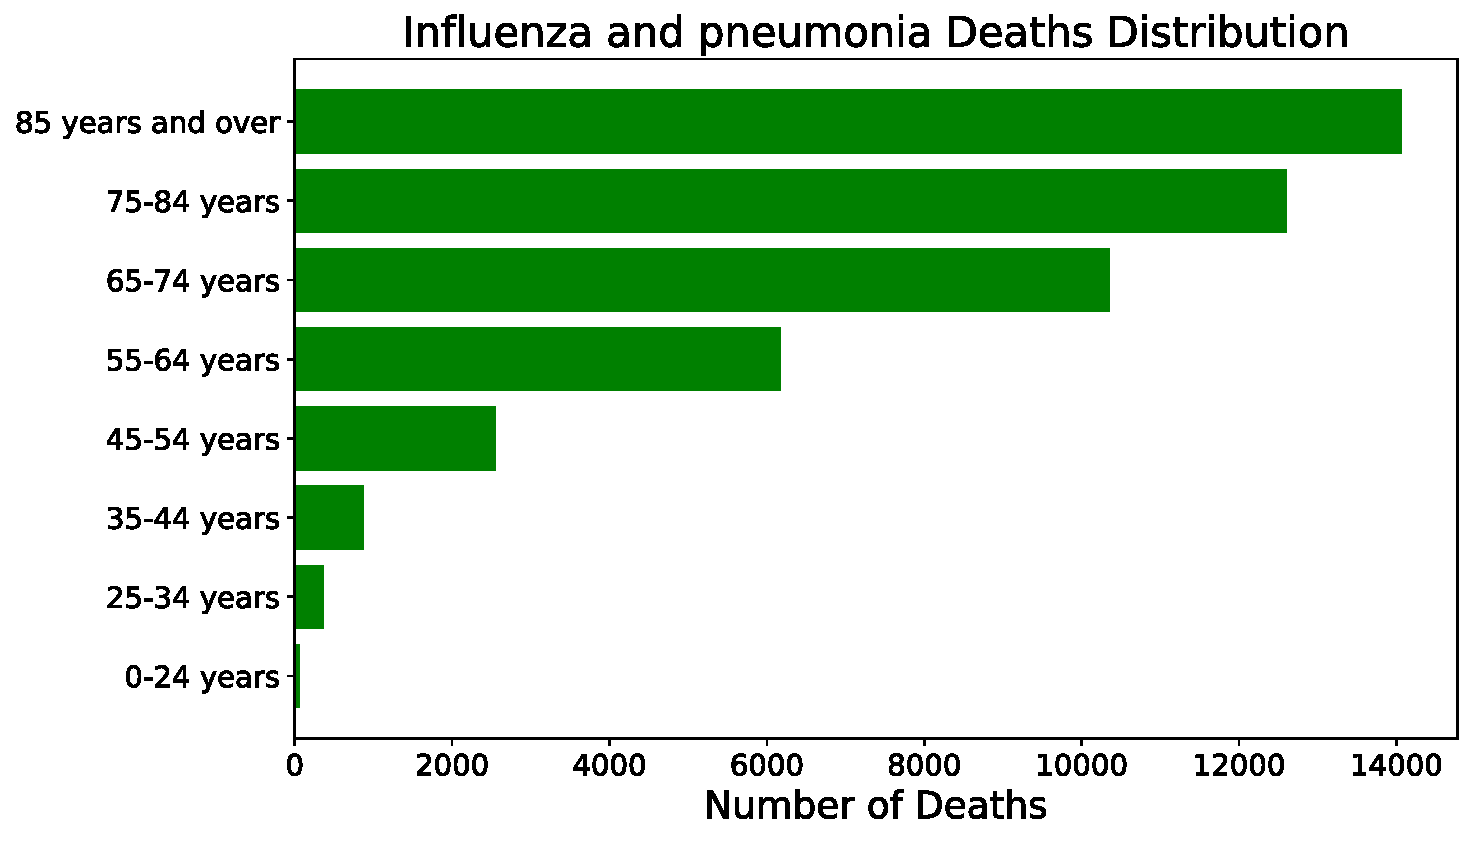
\includegraphics[width=0.65\linewidth]{latex/images/deaths_top.pdf}
    % 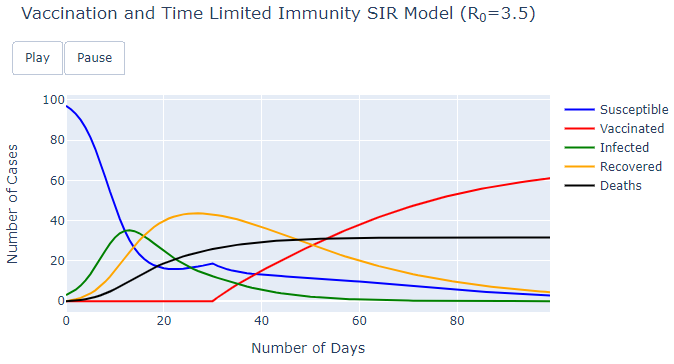
\includegraphics[width=13cm]{latex/images/vacc.PNG}%
    \vspace{-0.2cm}
    \caption{COVID-19 Deaths Distribution}
    \label{d_top}
\end{figure}